% You should title the file with a .tex extension (hw1.tex, for example)
\documentclass[11pt]{article}

\usepackage{amsmath}
\usepackage{amssymb}
\usepackage{fancyhdr}
\usepackage{isotope}
\usepackage{graphicx}
\graphicspath{{./images/}{./}}
\usepackage{array}

\oddsidemargin0cm
\topmargin-2cm     %I recommend adding these three lines to increase the 
\textwidth16.5cm   %amount of usable space on the page (and save trees)
\textheight23.5cm  

\newcommand{\question}[2] {\vspace{.25in} \hrule\vspace{0.5em}
\noindent{\bf #1: #2} \vspace{0.5em}
\hrule \vspace{.10in}}
\renewcommand{\part}[1] {\vspace{.10in} {\bf (#1)}}

\newcommand{\myname}{Matthew J. Urffer}
\newcommand{\myemail}{murffer@utk.edu}
\newcommand{\myhwnum}{1}

\pagestyle{fancyplain}
\lhead{\fancyplain{}{\textbf{HW\myhwnum}}}      % Note the different brackets!
\rhead{\fancyplain{}{\myname\\ \myemail}}
\chead{\fancyplain{}{CHEM-630}}

\begin{document}

\medskip                        % Skip a "medium" amount of space
                                % (latex determines what medium is)
                                % Also try: \bigskip, \littleskip

\thispagestyle{plain}
\begin{center}                  % Center the following lines
{\Large CHEM-630 Assignment \myhwnum} \\
\myname \\
\myemail \\
January 15, 2013 \\
\end{center}

\question{1.03}{Atoms}

\part{a} Look up the atomic numbers (Z) of Si, V, Re and Am
\begin{center}
\begin{tabular}{c | c}
Symbol & Z \\
\hline
\hline
Si & 14 \\
V & 23 \\
Re & 75 \\
Am & 95 \\
\end{tabular}
\end{center}

\part{b} Draw the structures for the three isotopes: \isotope[185]{Re}, \isotope[186]{Re} and \isotope[187]{Re}
\begin{center}
\begin{tabular}{m{2cm} m{5.1cm}}
\centering
Isotope & Structure \\
\hline
\hline
\isotope[185]{Re} & 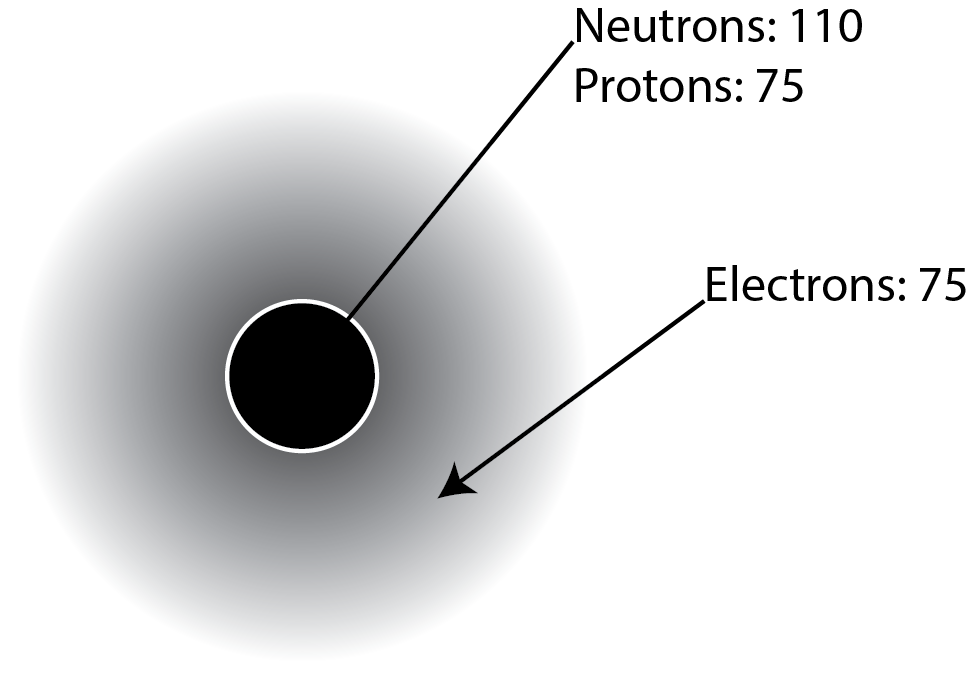
\includegraphics[width=5cm]{HW1_185Re.png} \\
\isotope[186]{Re} & 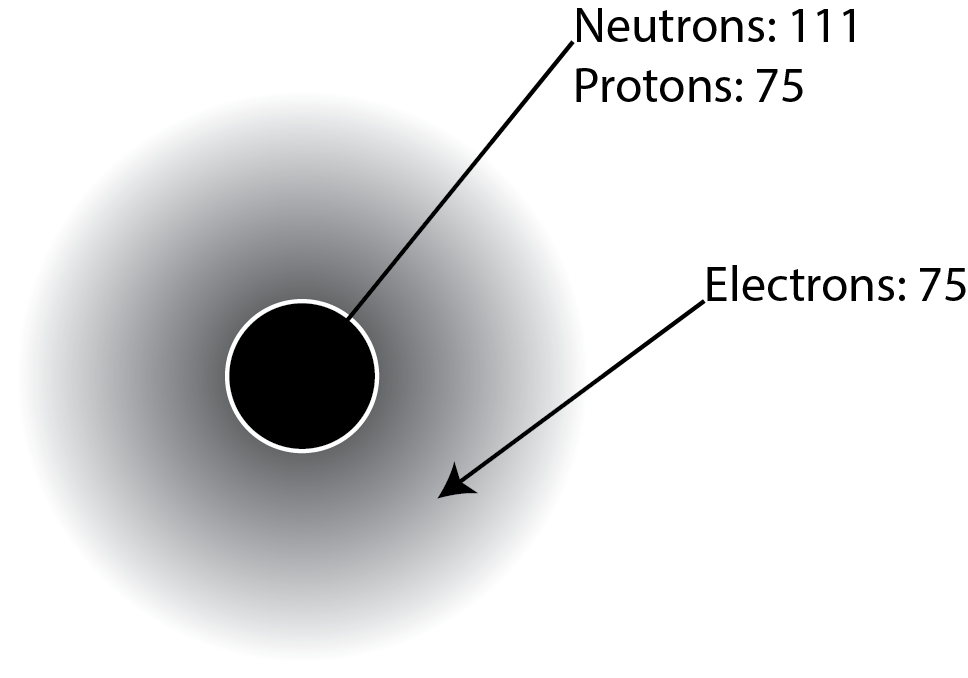
\includegraphics[width=5cm]{HW1_186Re.png} \\
\isotope[187]{Re} & 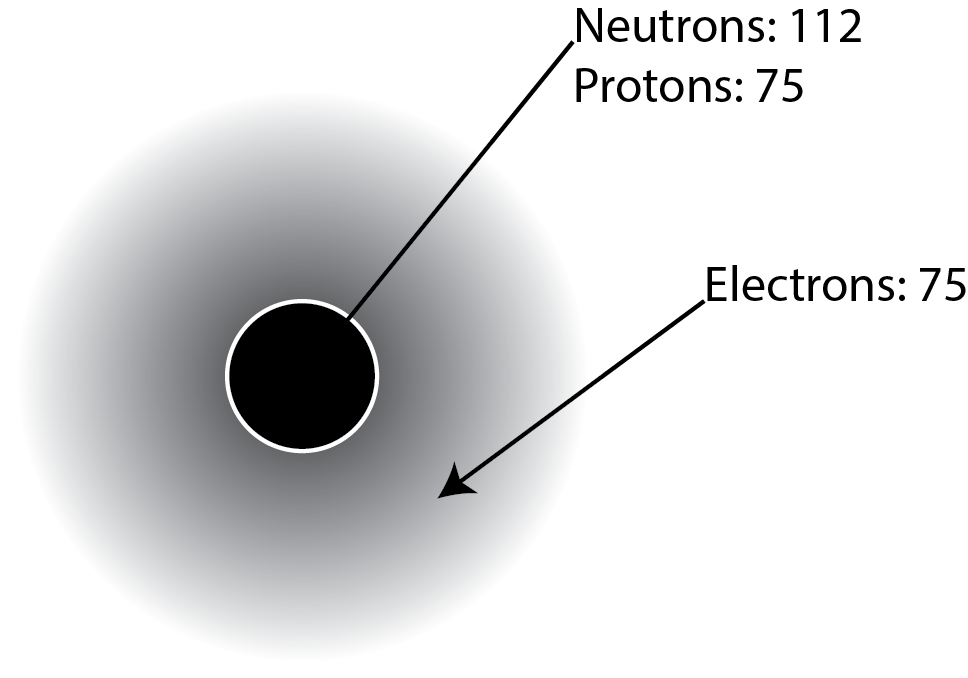
\includegraphics[width=5cm]{HW1_187Re.png} \\
\end{tabular}
\end{center}

\part{c} Write designations for the three isotopes in Part b in the form \isotope[A][Z]{El}
\begin{center}
\begin{tabular}{c c}
Isotope & Full Symbol \\
\hline
\hline
\isotope[185]{Re} & \isotope[185][75]{Re} \\ 
\isotope[186]{Re} & \isotope[186][75]{Re} \\ 
\isotope[187]{Re} & \isotope[187][75]{Re} \\ 
\end{tabular}
\end{center}

\part{d} Draw complete structures and give full symbols for \isotope[17]{O}, \isotope[126]{Dy} and \isotope[200]{Hg}
\begin{center}
\begin{tabular}{m{2cm} m{2cm} m{5.1cm}}
\centering
Isotope & Full Symbol & Structure \\
\hline
\hline
\isotope[17]{O} & \isotope[17][8]{O}      & 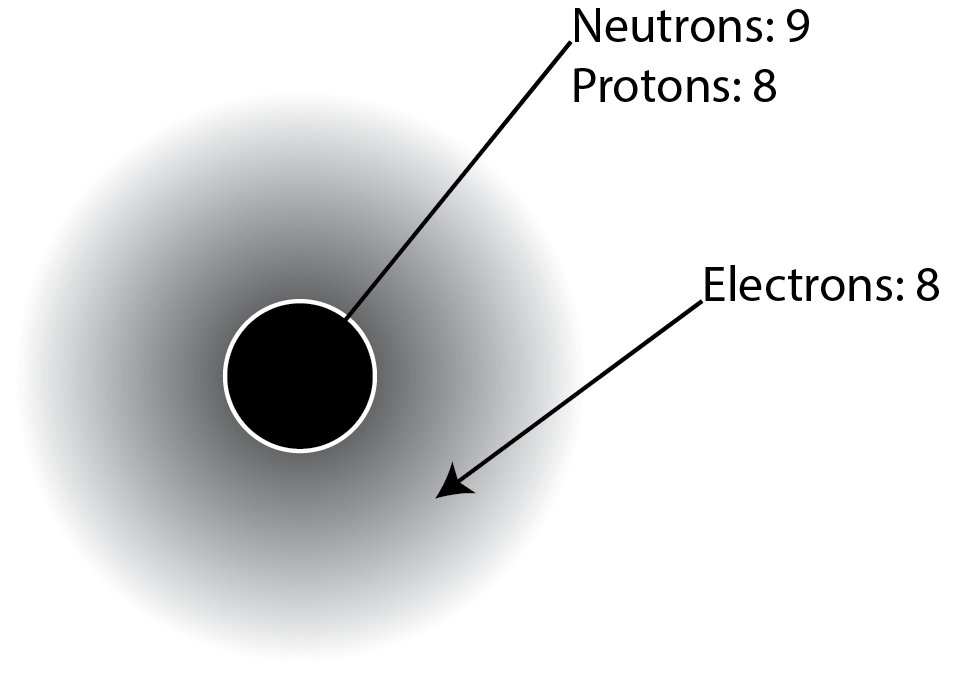
\includegraphics[width=5cm]{HW1_17O.png} \\
\isotope[126]{Dy} & \isotope[126][66]{Dy} & 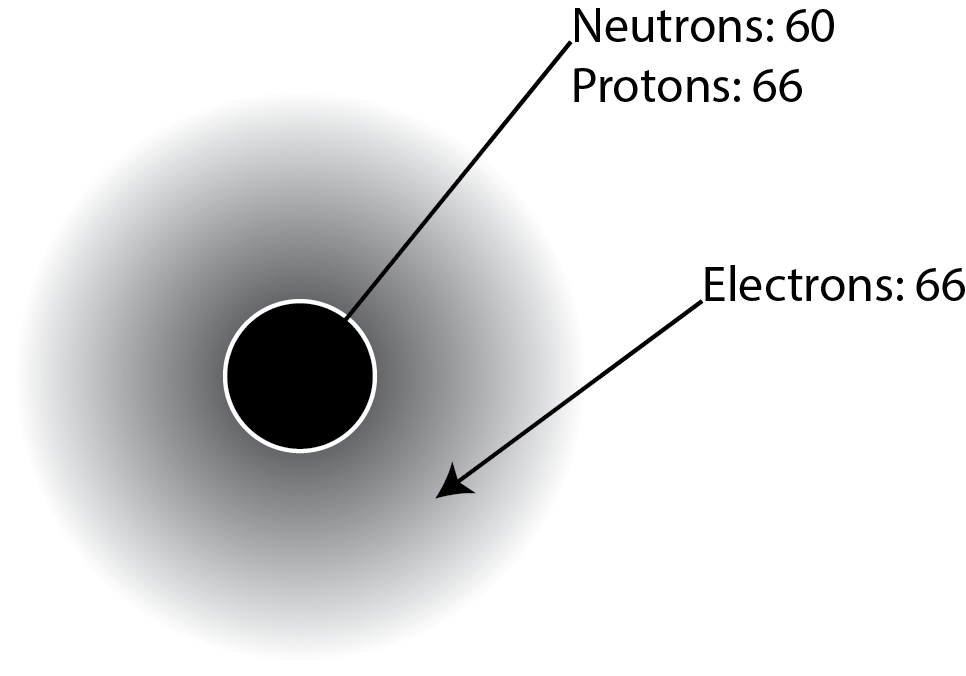
\includegraphics[width=5cm]{HW1_126Dy.png} \\
\isotope[200]{Hg} & \isotope[200][80]{Hg} & 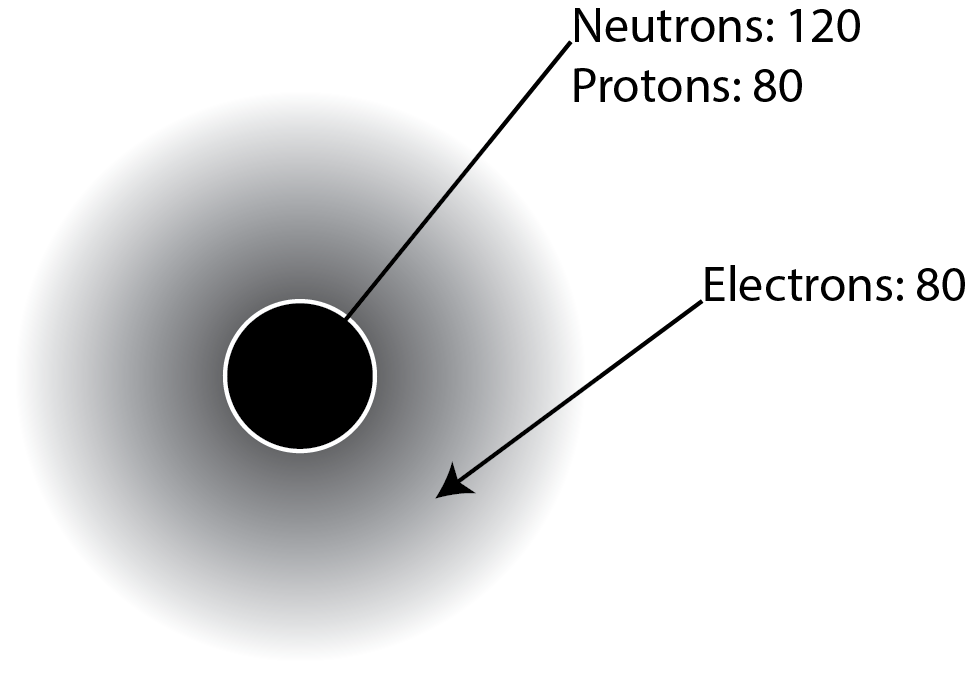
\includegraphics[width=5cm]{HW1_200Hg.png} \\
\end{tabular}
\end{center}

\question{Advanced Topic}{Extended Periodic Table}

The periodic table (a method of organizing elements while predicting properties and existence) was proposed by Dimitri Mendeleev in 1869. 
Since then, elements have been continuously added to the table.
Livermorium and Flerovium (\isotope[116]{Lv} \& \isotope[114]{Fl}) have become the most recent additions to the periodic table (May 31, 2012) while the 2010 discovery of ununseptium has yet to be verified.
The predictive properties of the periodic table have been used to aid in the search for elements, thus, the exact number of possible elements is an active research question.
Feynman calculated that elements with a Z greater than 137 the ground state energy of the 1s electron would become imaginary and thus oscillatory. This by itself does not rule out elements with a Z greater than 137, it just means that the atoms would be charged. 
In fact, when this calculation was revisited with a better model of the atom the 1s orbital energy remained positive until Z around 150.
A recent model of the periodic table has been created for Z $\le$ 172, based on updated computer models. These predicted, super heavy elements have been yet to be found, but have orbitals in the 6f and 5g, extending period 8.
\end{document}

